\documentclass[10pt,twocolumn,letterpaper]{article}

\usepackage{cvpr}
\usepackage{times}
\usepackage{epsfig}
\usepackage{graphicx}
\usepackage{amsmath}
\usepackage{amssymb}
\usepackage[encapsulated]{CJK} 

% Include other packages here, before hyperref.

% If you comment hyperref and then uncomment it, you should delete
% egpaper.aux before re-running latex.  (Or just hit 'q' on the first latex
% run, let it finish, and you should be clear).
\usepackage[breaklinks=true,bookmarks=false]{hyperref}

\cvprfinalcopy % *** Uncomment this line for the final submission

\def\cvprPaperID{****} % *** Enter the CVPR Paper ID here
\def\httilde{\mbox{\tt\raisebox{-.5ex}{\symbol{126}}}}

% Pages are numbered in submission mode, and unnumbered in camera-ready
%\ifcvprfinal\pagestyle{empty}\fi
\setcounter{page}{1}
\begin{document}
\begin{CJK}{UTF8}{bkai}
   %%%%%%%%% TITLE
   \title{Decoupling-NeRF: Decompose the scene and renderer in NeRF}

   \author{
      黃仁鴻\\
      P76094169\\
      NCKU CSIE
   }

   \maketitle
   %\thispagestyle{empty}

   %%%%%%%%% ABSTRACT
   % \begin{abstract}

   % \end{abstract}

   %%%%%%%%% BODY TEXT
   \section{Introduction}
   於 2020 年提出的神經輻射場(Neural Radiance Field,
   NeRF)~\cite{mildenhall2020nerf}利用簡單的類神經網路結構來擬和
   Volume Rendering 的 3D 模型。
   但 NeRF 的設計相當於是將 Renderer 與 Scene 嵌入於同一個類神經網路中,導致兩者具有高度耦合性而無法拆分。
   因此每當需要更換場景時,NeRF 就需要重新進行訓練。而不像一般訓練完之後就能套用在不同場景中的深度學習方法。

   然而在一般 3D 場景的儲存與展示,都是將 Scene 與 Renderer 拆分開來,並將 Scene
   作為輸入以取得對應視角的照片。這樣一來,Renderer 的部分就能重複利用於不同的
   3D 場景上。對應於原本 NeRF 中,訓練所使用的照片便相當於嵌入 NeRF
   之中的場景,若可以將照片改用於類神經網路的輸入,便等同將 Scene 與 Renderer 解耦合。

   因此,本次專題目標便是訓練出 Scene Encoder 對場景進行編碼照片,並使用 Multi Head Attention~\cite{AttentionIsAllYouNeed}
   將其重新組建為 View Embedding,最後透過單一 Neural Renderer 生成場景照片。


   \begin{figure}[t]
      \begin{center}
         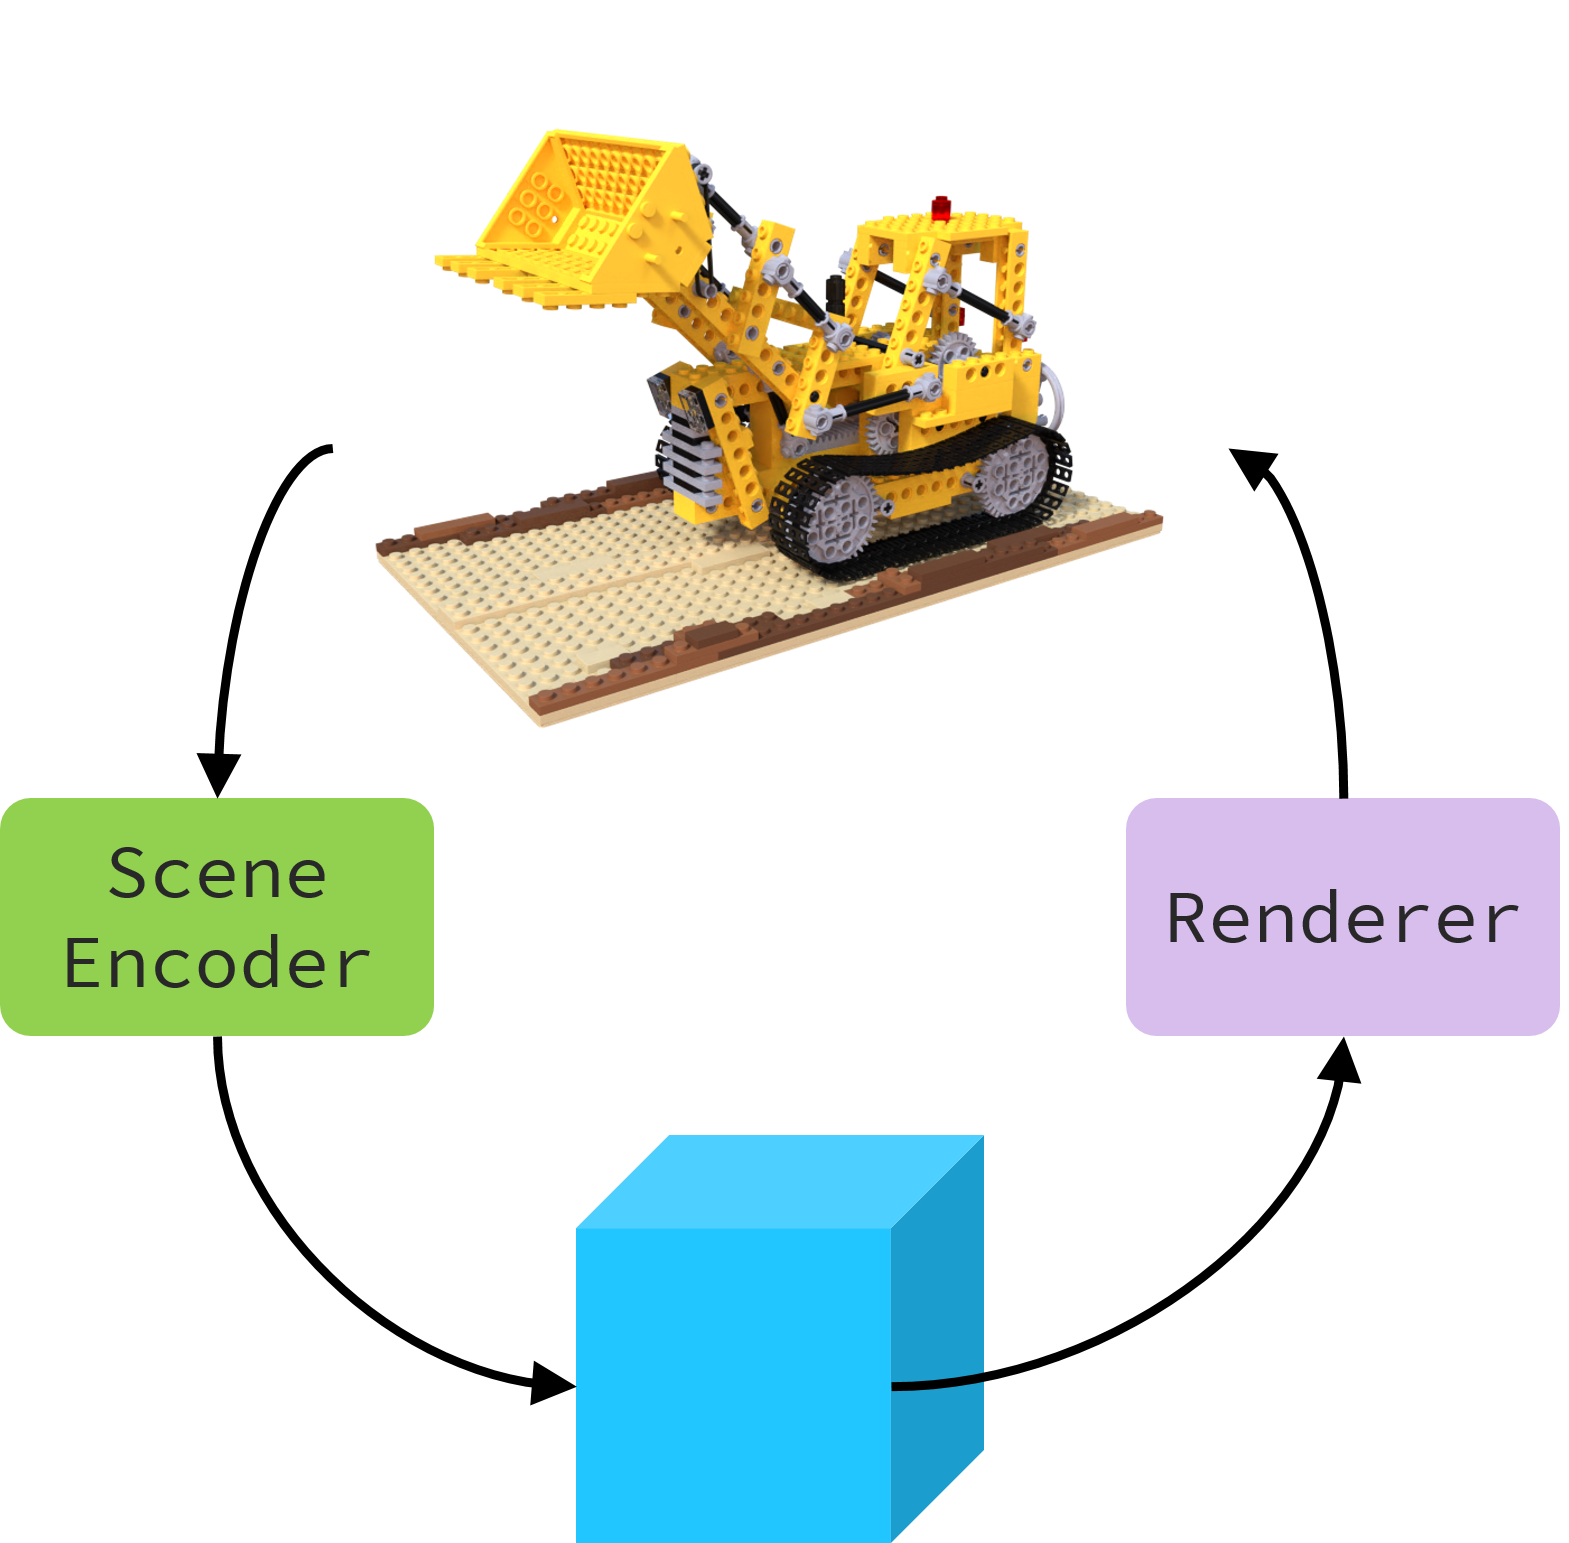
\includegraphics[width=1\linewidth]{img/auto-encoder.png}
      \end{center}
      \caption{
         預先訓練 Auto Encoder。
      }
      \label{fig:auto-encoder}
   \end{figure}

   \begin{figure}[t]
      \begin{center}
         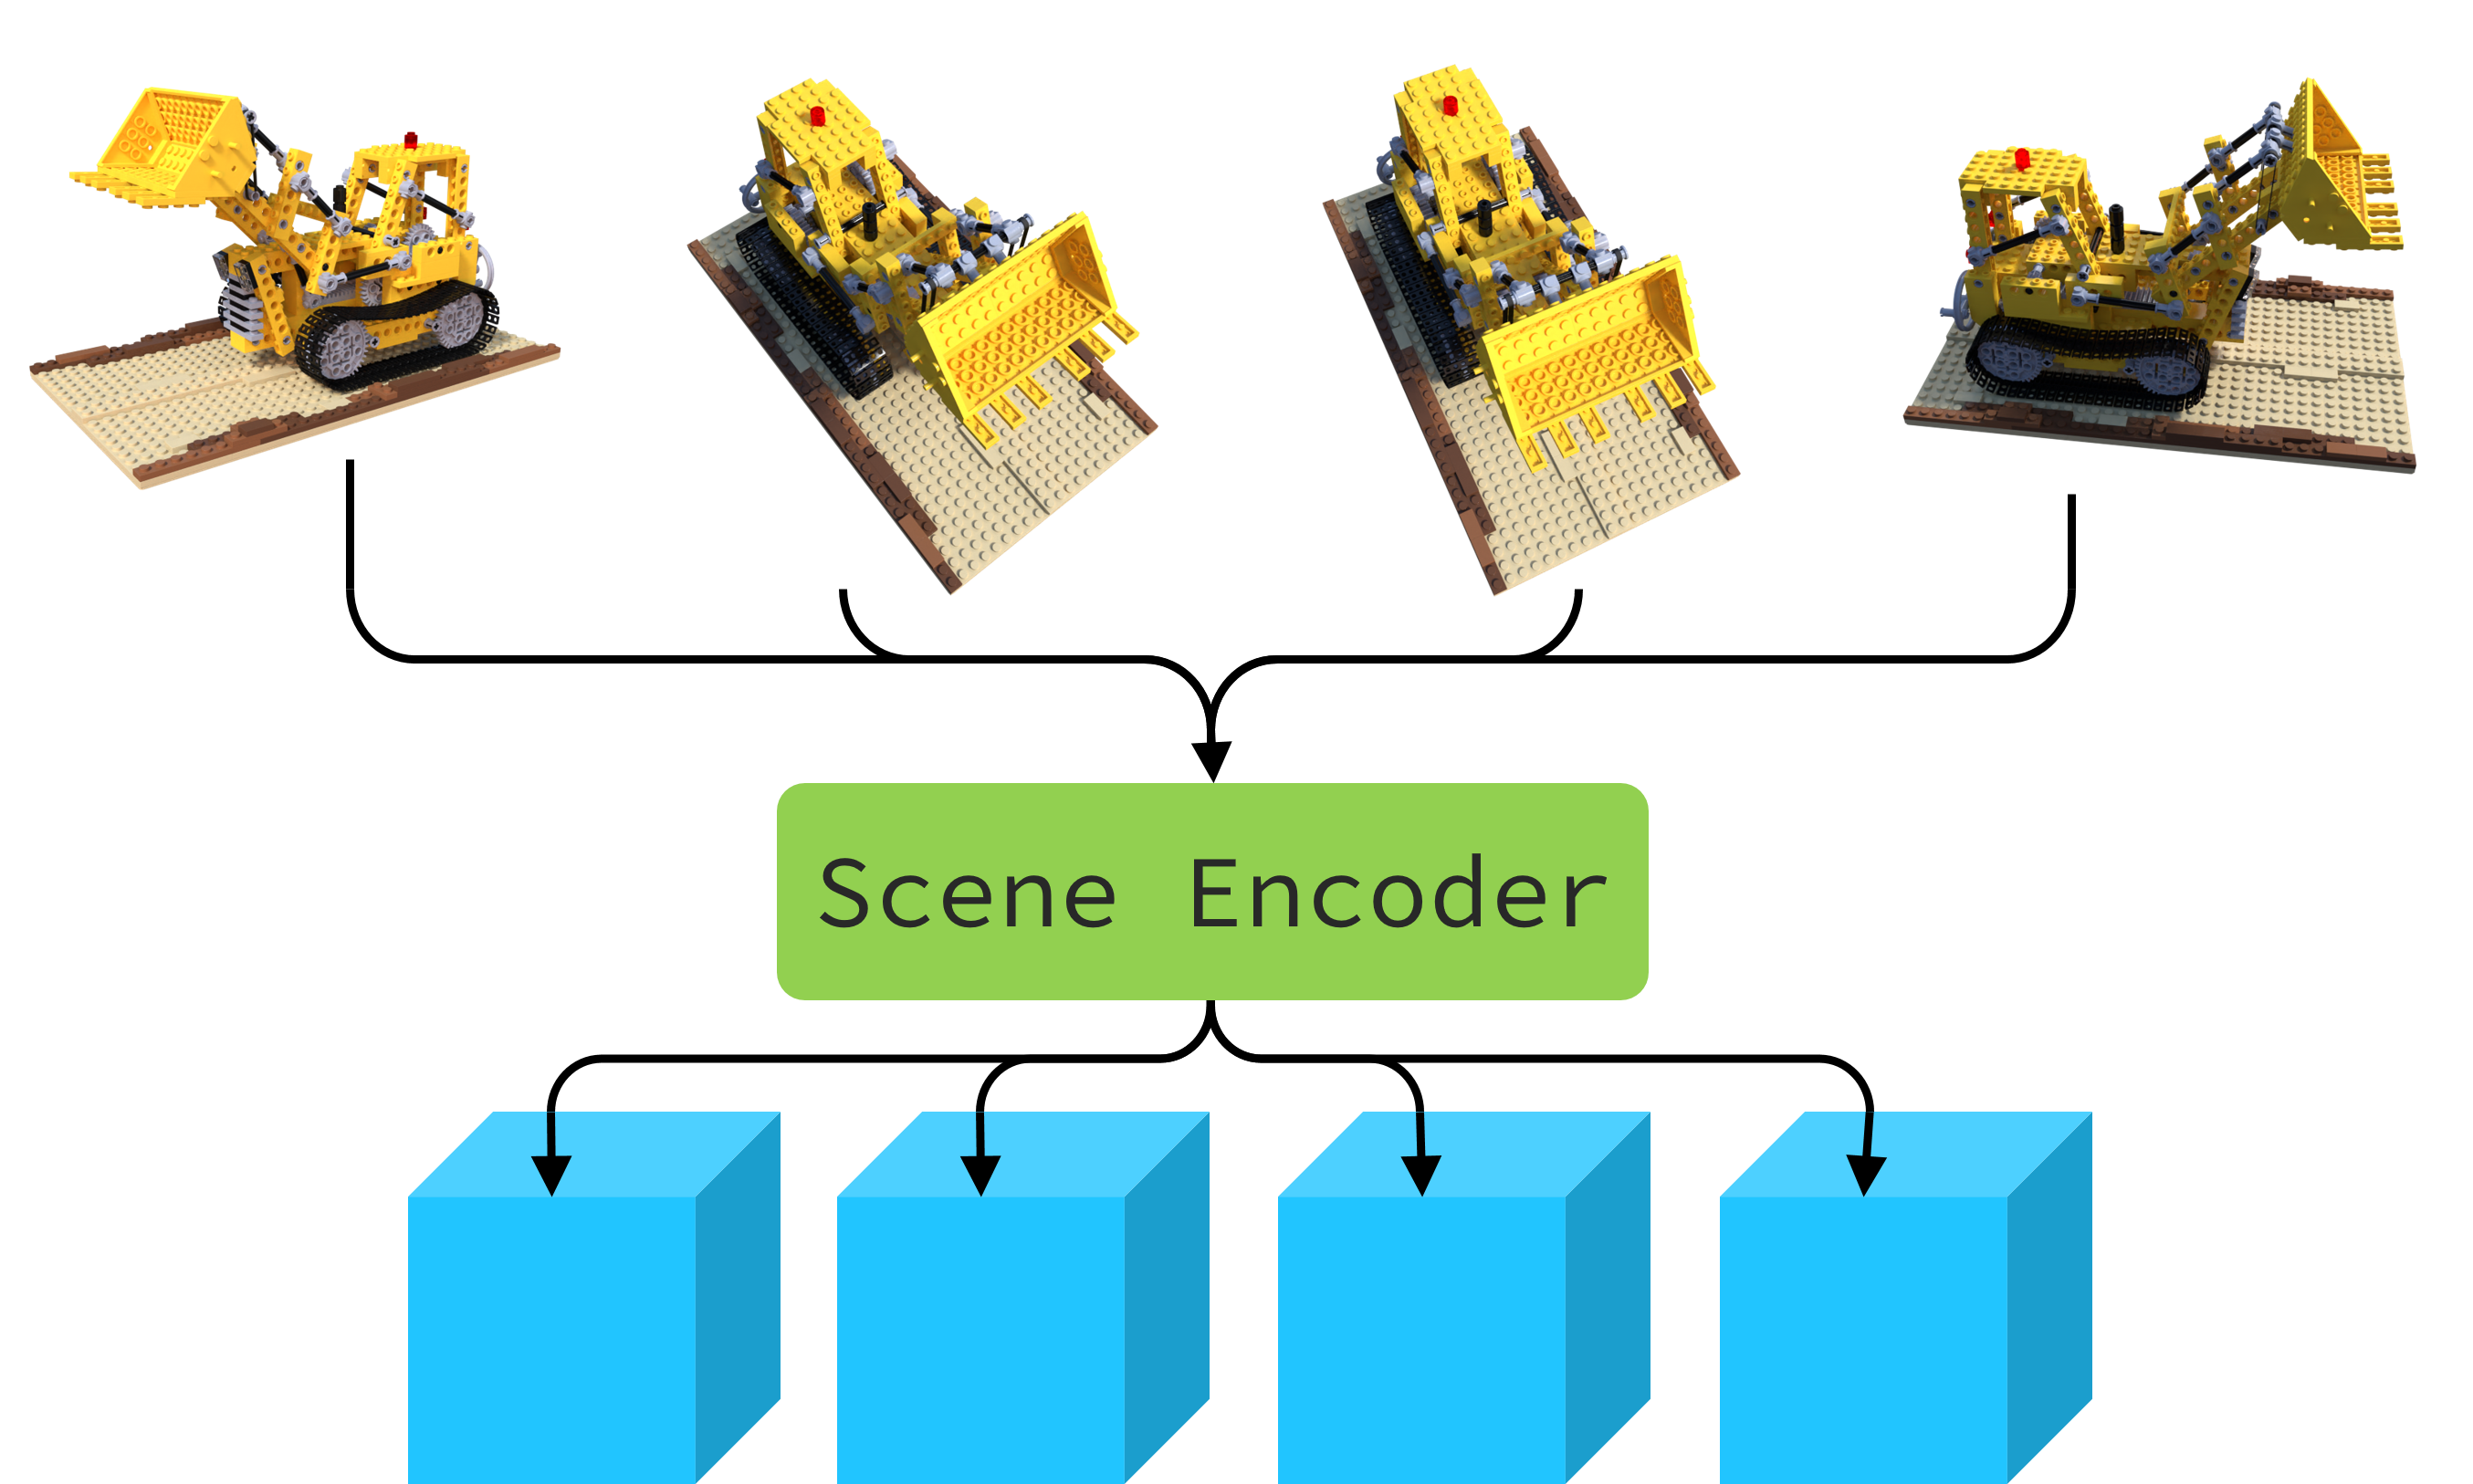
\includegraphics[width=1\linewidth]{img/encode-scene.png}
      \end{center}
      \caption{
         將場景照片透過 Encoder 編碼成 Scene Embedding。
      }
      \label{fig:encode-scene}
   \end{figure}

   \begin{figure*}
      \begin{center}
         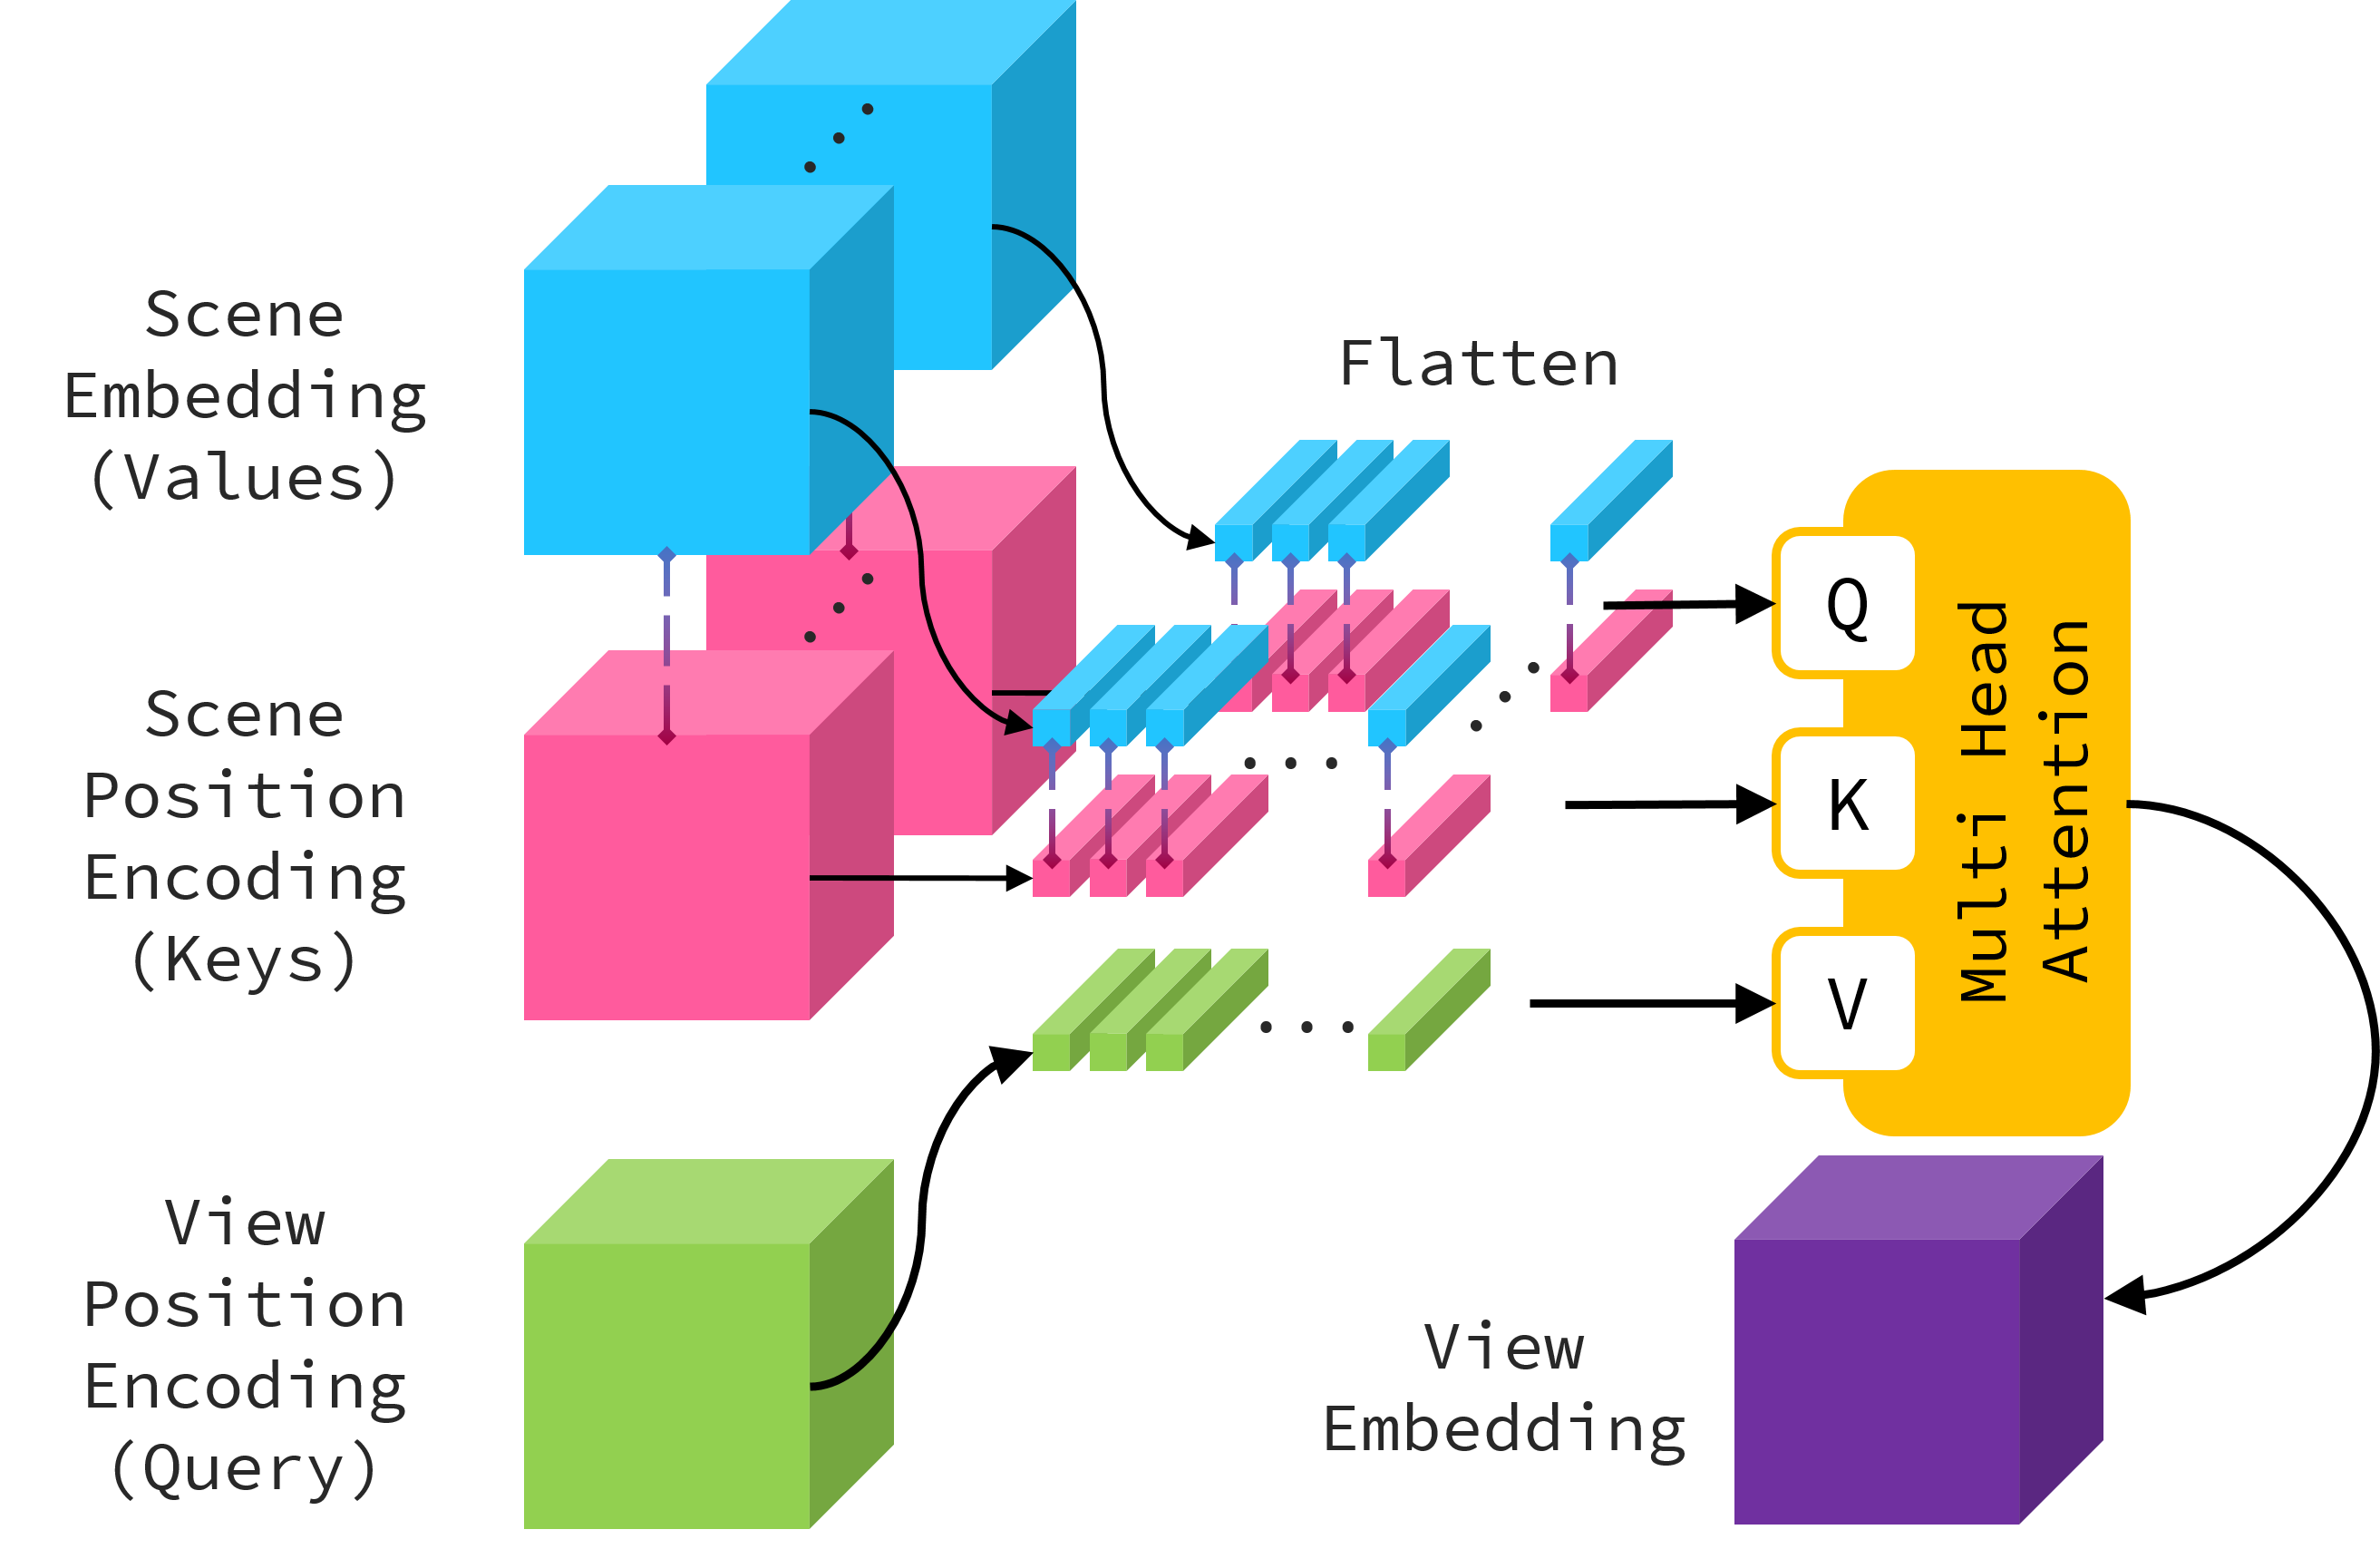
\includegraphics[width=1\linewidth]{img/view-embedding.png}
      \end{center}
      \caption{
         將目標視角的位置編碼作為 Querys,與 Scene Embedding 及其對應的位置編碼計算
         Multi Head Attention 來取得 View Embedding。
      }
      \label{fig:view-embedding}
   \end{figure*}

   \begin{figure}[t]
      \begin{center}
         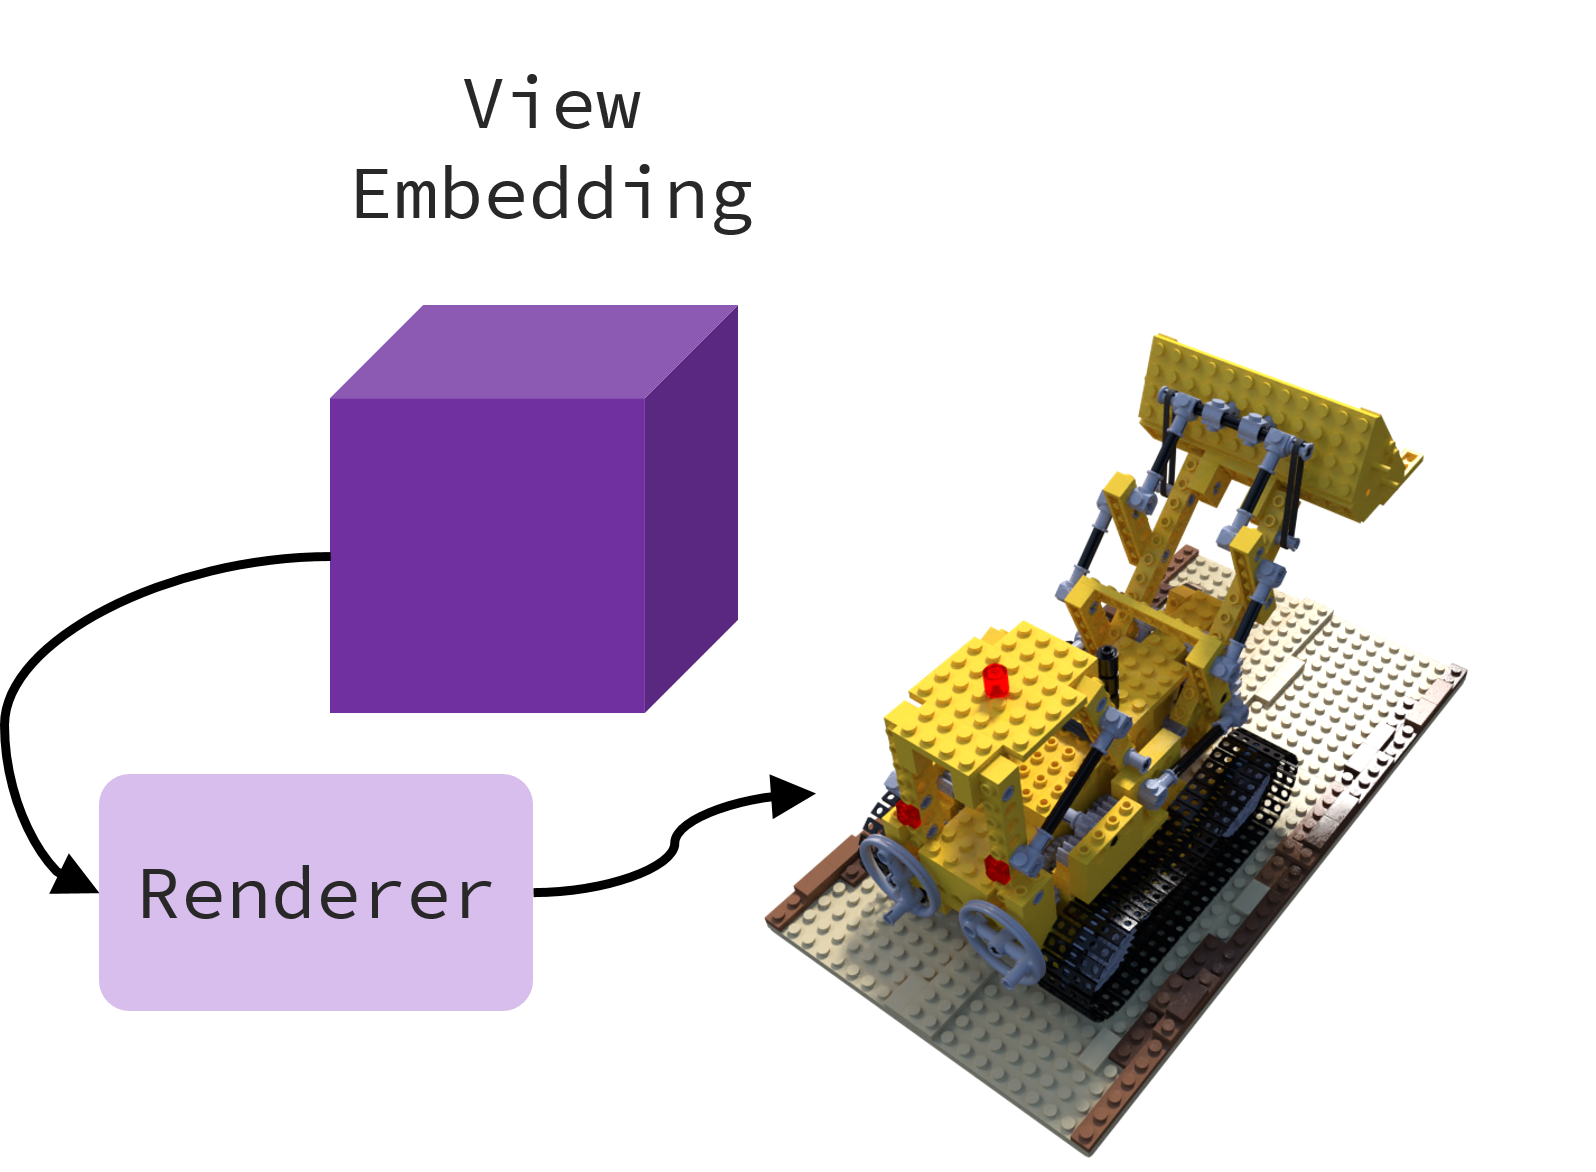
\includegraphics[width=1\linewidth]{img/render-view.png}
      \end{center}
      \caption{
         將 Figures~\ref{fig:view-embedding} 得到的 View Embedding 交由
         Renderer 進行 Volume Rendering。
      }
      \label{fig:render-view}
   \end{figure}
   %------------------------------------------------------------------------
   \section{System framework}
   本專題訓練會區分成兩步驟,第一步如同 Figures~\ref{fig:auto-encoder}
   所示,預訓練用於生成 Scene Embedding 與 Render 的
   AutoEncoder。Figures~\ref{fig:view-embedding} 則代表第二步驟,訓練重構
   View Embedding 的 Multi Head Attention Block
   並再次調整第一步所獲得之 Renderer。

   像是 Figures~\ref{fig:encode-scene} 中所示,先利用 Encoder 將少量圖片轉換成 Scene
   Embedding。而在 Figures~\ref{fig:view-embedding},每個 Embedding 皆會依據各自的拍攝角度、位置得到相對應的
   Scene Position Encoding。再重構 View Embedding 時,便要先將拍攝視角轉換成 View Position
   Encoding,並配合
   其中,進入 Multi Head Attention Block 的資訊

   本專題使用的模型結構如 是由 Encoder 與 Decoder 兩區塊組合而成,
   其中負責抽取語音特徵 Encoder 區塊將會使用 BYOL 與 SimSiam 進行預訓練。
   在進行 CL 訓練時,語音 $S$ 會混合 $N_1$ 與 $N_2$ 兩個不同的噪音後,輸入 Encoder
   取出語音的特徵向量,並用 Figure 2. 與 Figure 3. 所述的方法更新其內部權重\footnote{
      在 Figure 2. 與 Figure 3. 中的 X 符號代表 Stop Gradient,因此梯度並不會通過該區段向前更新。}。

   在使用 CL 預訓練完 Encoder~\ref{fig:view-embedding} 後,便會將其串接上
   Decoder,將乾淨的語音當成目標來進行語音增強任務的學習。更詳細的實驗內容在 Expected results 中。


   %------------------------------------------------------------------------
   \section{Expected results}
   本專題使用的噪音資料集是由 20 種不同類型的背景噪音所組成,總共有 100 個音檔的 Nonspeech~\cite{mildenhall2020nerf}。
   而語音資料集則是選用 TIMIT~\cite{mildenhall2020nerf},TIMIT 具有 6300 句語音,這些語音包含美國八個地區共 630 人所念出的 10
   個指定句子。在訓練時的噪聲語音是將 TIMIT 與 Nonspeech 以 -5, 0, 5 這三種 SNR 混合產生的。


   % 本專題分別使用 TIMIT~\cite{timit} 與 Nonspeech~\cite{Nonspeech}
   % 作為語音和雜訊的資料集,並以 -5, 0, 5 這三種 SNR 混合成的噪聲語音當模型輸入。
   % Nonspeech 是由 20 種不同類型的背景噪音所組成,總共有 100
   % 個音檔,而 TIMIT 則為 6300 句語音組成資料集,這些語音包含美國八個地區共 630 人所念出的 10
   % 個指定句子。

   本專題預計將會進行以下幾項實驗:
   \begin{enumerate}
      \item 直接對 AutoEncoder 訓練 Speech Enhancement 任務。
      \item 基於 BYOL 對 Encoder 與 Bottleneck 進行預訓練後凍結參數,然後接上 Decoder 訓練 Speech Enhancement 任務。
      \item 基於 SimSiam 對 Encoder 與 Bottleneck 進行預訓練後凍結參數,然後接上 Decoder 訓練 Speech Enhancement 任務。
      \item 將 BYOL 訓練得到的參數作為初始權重後,對 AutoEncoder 訓練 Speech Enhancement 任務。
      \item 將 SimSiam 訓練得到的參數作為初始權重後,對 AutoEncoder 訓練 Speech Enhancement 任務。
      \item 基於不同數量的樣本進行上述實驗,以測試各種方法的泛化能力。
   \end{enumerate}

   最終將比較上述不同方法所訓練得到模型的 PESQ\cite{mildenhall2020nerf}、STOI\cite{mildenhall2020nerf} 與 SISDR\cite{mildenhall2020nerf}。


   {\small
   \bibliographystyle{ieee_fullname}
   \bibliography{egbib}
   }
\end{CJK}
\end{document}
